\chapter{Kombinatorické identity}

Nyní jsme si již prošli základní nástroje, které v kombinatorice využíváme. V rámci minulé kapitoly jsme si ukázali práci s kombinačními čísly a především jejich význam. Nyní se na ně trochu více zaměříme, neboť zjistíme, že tento matematický objekt má pozoruhodné vlastnosti, díky kterým obdržíme několik zajímavých identit.

\section{Vlastnosti kombinačních čísel}

V této sekci se budeme \emph{především} (avšak ne vždy) držet naší původní definice kombinačního čísla z \ref{def:kombinacni_cislo}, tj.
\[\binom{n}{k}=\dfrac{n(n-1)(n-2)\cdots(n-k+1)}{k!},\]
a to právě kvůli již zmíněné vlastnosti, že oproti
\[\dfrac{n!}{(n-k)!k!}\]
dává výraz smysl i pro $k>n$ a je vždy roven nule (ostatně i z kombinatorického hlediska dává tento výsledek smysl). Nebudeme se tak muset explicitně odvolávat na předpoklad, že $n\leqslant k$, abychom předešli formálním nepřesnostem.
\medskip

U kombinačních čísel lze pozorovat některé zajímavé vlastnosti. Začneme asi tou nejzákladnější.
\begin{theorem}[Symetrie kombinačních čísel]
    Pro $n,\,k\in\N_0$, kde $k\leqslant n$, platí
    \[\binom{n}{k}=\binom{n}{n-k}.\]
\end{theorem}
\begin{proof}[Důkaz první]
    Asi nejjednodušší důkaz je přímým výpočtem:
    \[\binom{n}{n-k}=\dfrac{n!}{(n-(n-k))(n-k)!}=\dfrac{n!}{k!(n-k)!}=\binom{n}{k}.\]
\end{proof}
\begin{proof}[Důkaz druhý]
    Názornější důkaz nám poskytne kombinatorická interpretace tohoto tvrzení. Libovolná $k$-tice (v tomto smyslu množina) je jednoznačně určena výběrem prvků z nějaké $n$ prvkové množiny, které jí budou náležet. Výběrem $k$ prvků z dané množiny tak zbude $n-k$ prvků, které nejsou součástí dané $k$-tice.
    \todo{obrázek}
\end{proof}
\section{Binomická věta}

Kombinační čísla mají kromě kombinatorických úloh využití i v klasické aritmetice. Ať už se to zdá, nebo ne, tyto dva možná zdánlivě rozdílné světy si nejsou až tak vzdálené. V této sekci se proto podíváme na větu, která nám trochu více zobecní koncept roznásobování dvojčlenů.\par
Podívejme se nejdříve na ty nejjednodušší případy:
\begin{align*}
    (x+y)^0&=1,\\
    (x+y)^1&=x+y,\\
    (x+y)^2&=x^2+2xy+y^2,\\
    (x+y)^3&=x^3+3x^2y+3xy^2+y^3,\\
    (x+y)^4&=x^4+4x^3y+6x^2y^2+4xy^3+y^4,\\
    &\vdots
\end{align*}
Čeho bychom si mohli na poprvé možná všimnout je faktu, že koeficienty u jednotlivých členů jsou symetrické. To je asi nejlépe vidět u roznásobení čtvrté mocniny dvojčlenu $x+y$. Proč tomu ale tak je? Vzpomeňme si na větu \ref{thm:symetrie_kombinacnich_cisel}, díky které jsme se dozvěděli, že kombinační čísla jsou "symetrická", tzn. $\binom{n}{k}=\binom{n}{n-k}$. Další pozorování bychom z tohoto zápisu učili nejspíše stěží (avšak klobouček dolů všem, kteří to již vidí :-)). Zkusme se zaměřit nyní čistě na dané koeficienty. Počet členů je vždy totiž lichý, což nám umožňuje zapsat si jejich koeficienty ve schématu níže.
\begin{figure}[H]
    \centering
    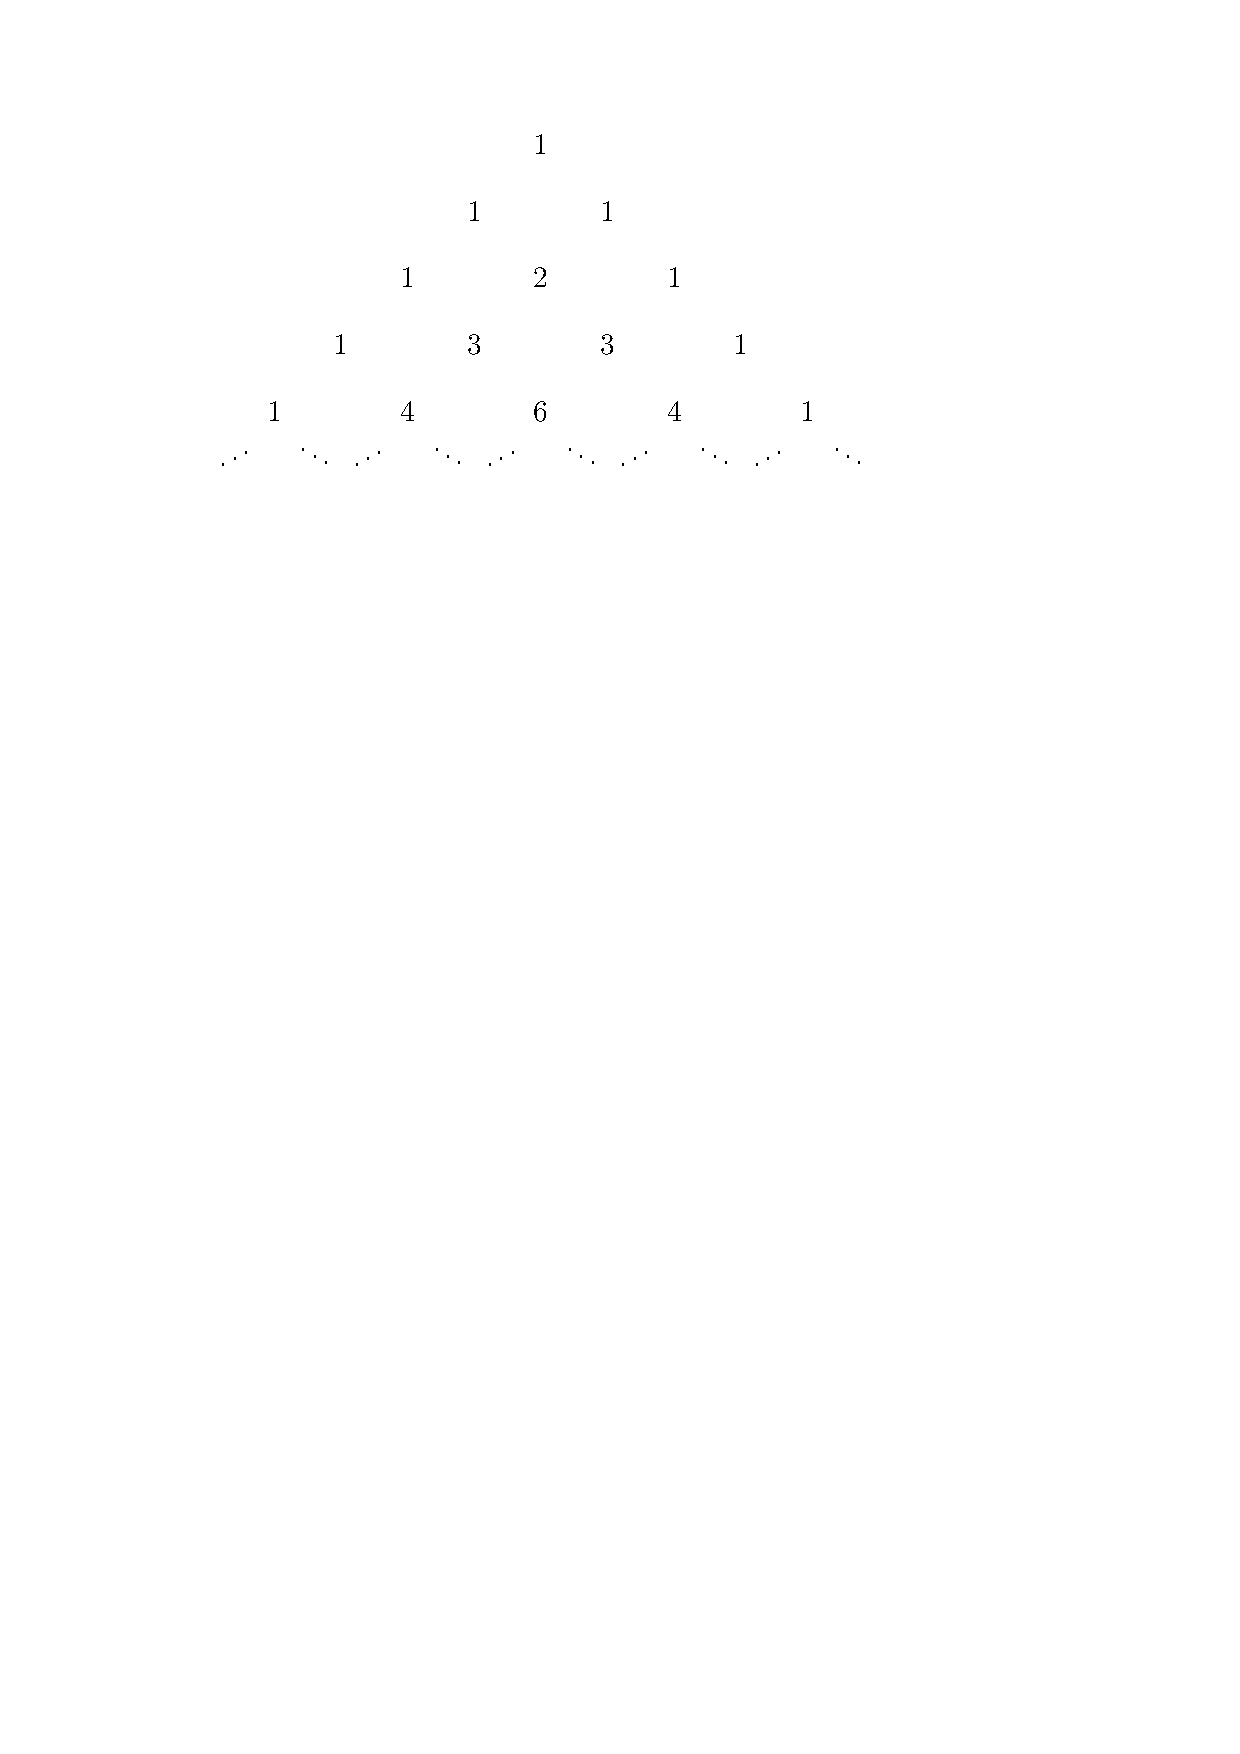
\includegraphics[scale=\normalipe]{ch03_pascaluv_trojuhelnik.pdf}
    \caption{Schéma koeficientů ve tvaru pyramidy.}
    \label{fig:pascaluv_trojuhelnik}
\end{figure}
Toto schéma se nazývá \textbf{Pascalův trojúhelník}. Pokud se podíváme blíže, lze si všimnout, jak vznikají jeho řádky. Na kraji vždy pevně stojí číslo 1 a další koeficienty vzniknou součtem koeficientů nad ním.
\begin{figure}[H]
    \centering
    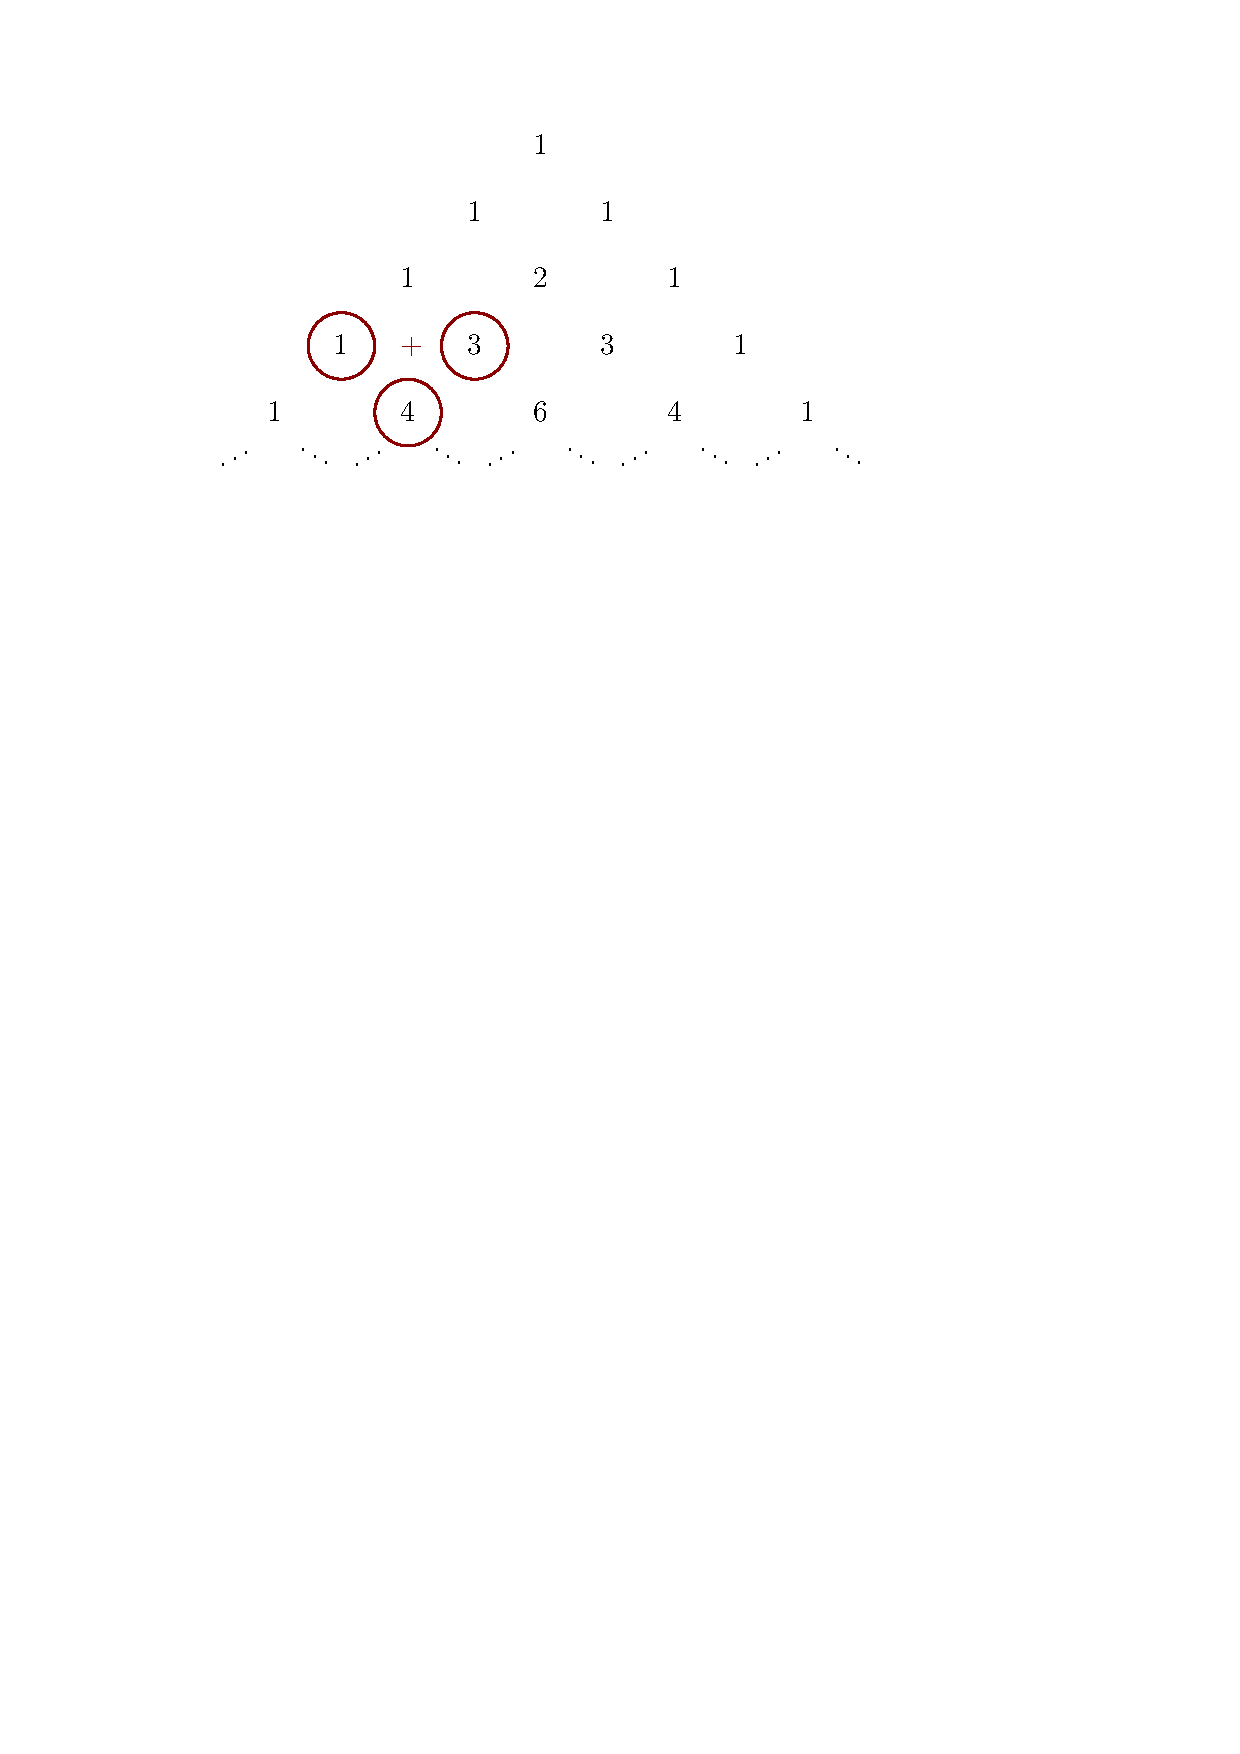
\includegraphics[scale=\normalipe]{ch03_pascaluv_trojuhelnik_soucet.pdf}
    \caption{Generování Pascalova trojúhelníku součtem členů.}
    \label{fig:pascaluv_trojuhelnik_soucet}
\end{figure}
Pokud se nyní vrátíme opět ke kombinačním číslům, jistě si vzpomeneme, že jsme zde měli větu \ref{thm:soucet_kombinacnich_cisel}, která dávala do souvislosti kombinační čísla a jejich součet. Z toho by nás tak mohlo napadnout, že jednotlivá čísla v Pascalově trojúhelníku by tak mohla odpovídat jistým kombinačním číslům. Je tomu skutečně tak.
\begin{figure}[H]
    \centering
    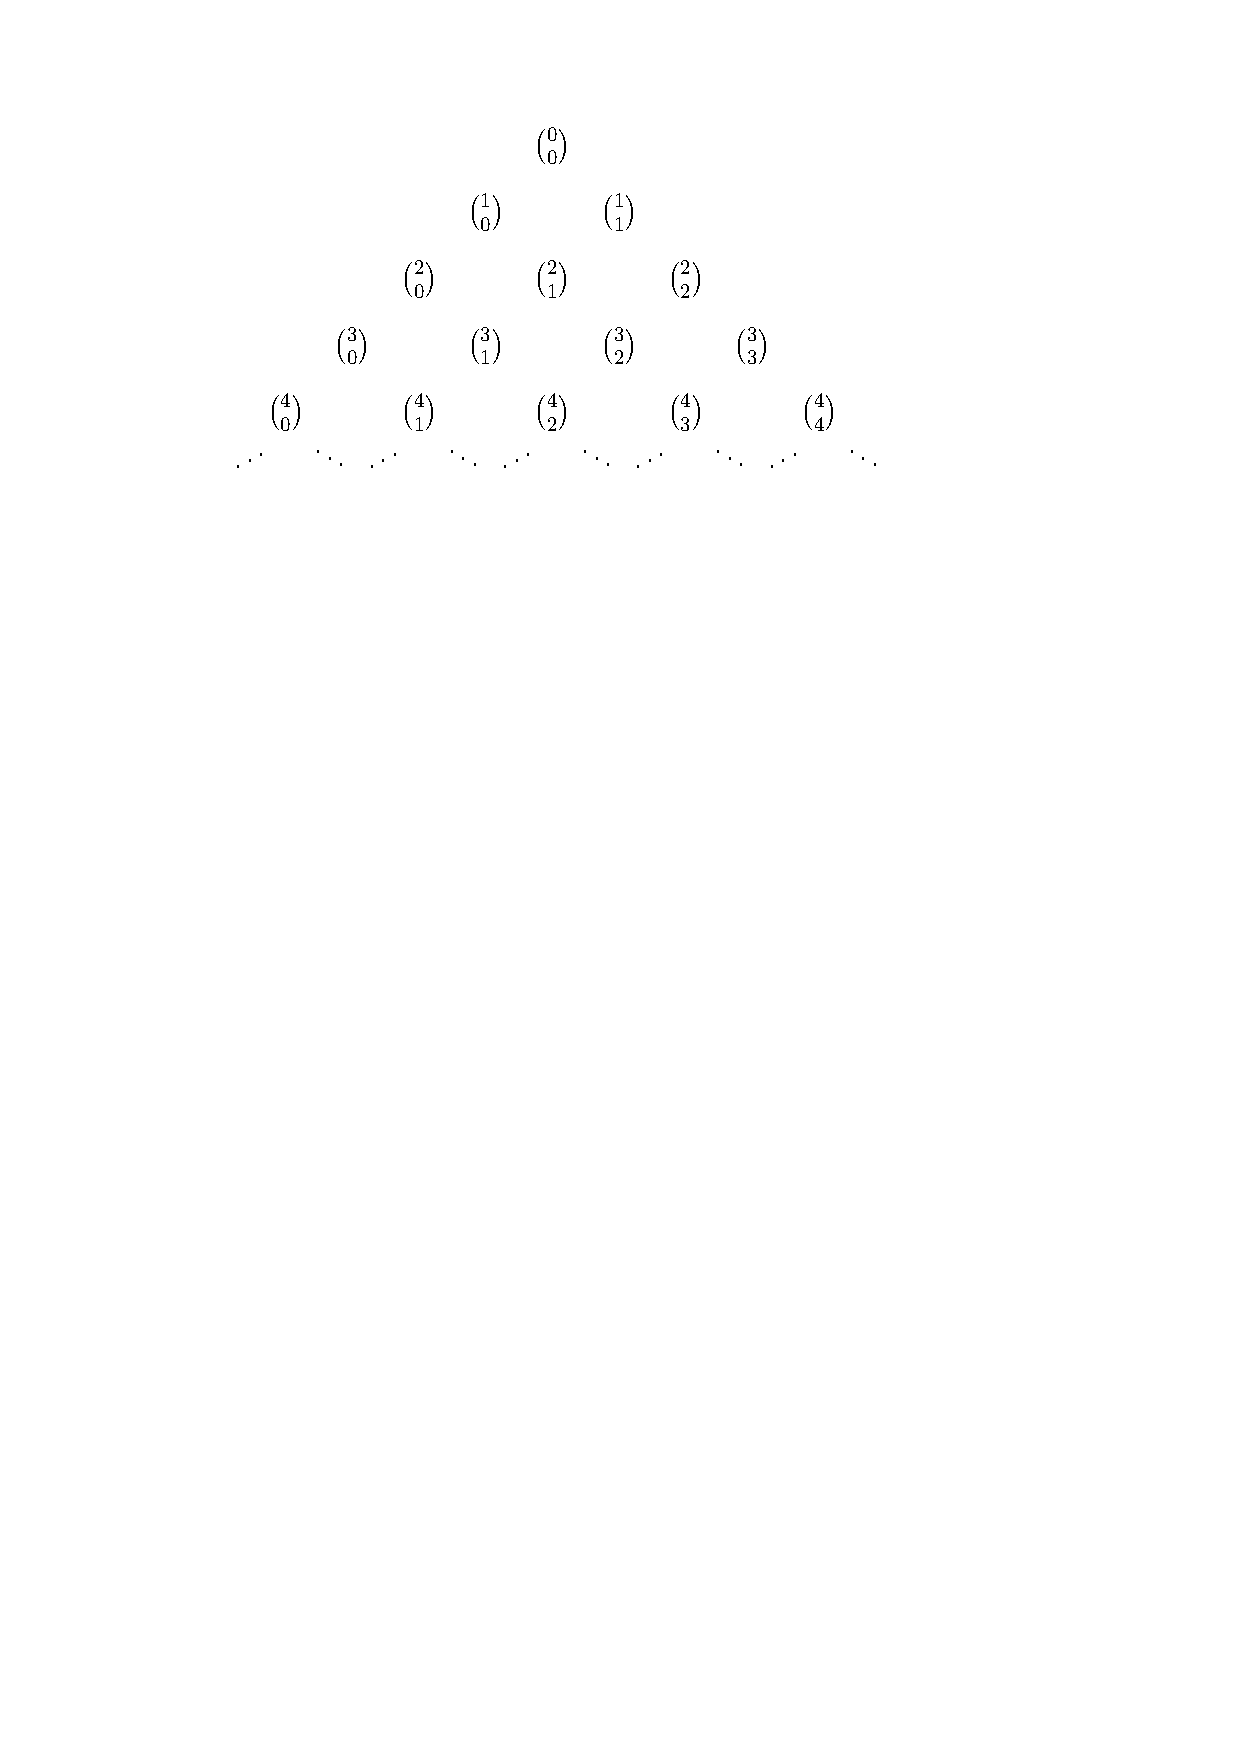
\includegraphics[scale=\normalipe]{ch03_pascaluv_trojuhelnik_kombinacni_cisla.pdf}
    \caption{Pascalův trojúhelník pomocí kombinačních čísel.}
    \label{fig:pascaluv_trojuhelnik_kombinacni_cisla}
\end{figure}
Sami se můžete přesvědčit, že jednotlivá kombinační čísla odpovídají daným koeficientům. Navíc zde lze i vidět i jejich další vlastnosti v uplatnění, konkrétně věty \ref{thm:symetrie_kombinacnich_cisel} (stačí se podívat na $k$-tý člen a příslušném $(n-k)$-tý člen, kde $n$ zde představuje číslo řádku od nuly, neboť odpovídá mocnině daném dvojčlenu) a \ref{thm:soucet_kombinacnich_cisel} (koeficient různý od jedničky na kraji je součtem koeficientů nad ním).\par

Vraťme se nyní k roznásobování dvojčlenů. Z Pascalova trojúhelníku lze tak vidět, že koeficienty v rozvoji $(x+y)^n$ by mohly být po řadě čísla
\[\binom{n}{0},\,\binom{n}{1},\,\binom{n}{2},\,\cdots,\,\binom{n}{n}.\]
Jak lze ukázat, platí totiž následující věta.
\begin{theorem}[Binomická]\label{thm:binomicka_veta}
    Pro libovolná $x,\,y\in\C$ a $n\in\N$ platí
    \[(x+y)^n=\sum_{k=0}^{n}\binom{n}{k}x^{n-k}y^k,\]
    neboli
    \[(x+y)^n=\binom{n}{0}x^ny^0+\binom{n}{1}x^{n-1}y^1+\binom{n}{2}x^{n-2}y^2+\cdots+\binom{n}{n}x^0y^n.\]
\end{theorem}
\begin{proof}
    Nejnázornějším důkazem pro nás opět bude kombinatorická úvaha. Rozepišme si součin $(x+y)^n$ jako
    \[\underbrace{(x+y)(x+y)\cdots(x+y)}_{n\text{-krát}}.\]
    Sečíst můžeme pouze členy, které mají v součinu stejný počet $x$ a stejný počet $y$. Např.
    \[(x+y)(x+y)(x+y)=xxx+xxy+xyx+yxx+xyy+yxy+yyx+yyy=x^3+3x^2y+3xy^2+y^3.\]
    Člen $x^{n-k}y^k$ tvoří tak uspořádanou $n$-tici činitelů z $x$ a $y$.
    \[\underbrace{x\cdot x\cdots x}_{(n-k)\text{-krát}} \cdot \underbrace{y\cdot y\cdots y}_{k\text{-krát}}.\]
    Takovou uspořádanou $n$-tici můžeme sestavit tak, že vybereme $k$ pozic pro činitel $y$ (zbylých $n-k$ pozic doplníme činitelem $x$). Takových výběrů existuje $\binom{n}{k}$, a tedy v tomto počtu se daný člen objeví v rozvoji $(x+y)^n$.
\end{proof}
\begin{task}
    Vypočítejte rozvoj $\displaystyle \left(x+\dfrac{1}{2y}\right)^5$.
\end{task}
\begin{solution}
    Postupujeme podle binomické věty \ref{thm:binomicka_veta}:
    \begin{align*}
        \left(x+\dfrac{1}{2y}\right)^5 &\stackrel{\ref{thm:binomicka_veta}}{=}\sum_{k=0}^{5}\binom{5}{k}x^{5-k}\left(\dfrac{1}{2y}\right)^k \\
        &=\binom{5}{0}x^5\left(\dfrac{1}{2y}\right)^0+\binom{5}{1}x^4\left(\dfrac{1}{2y}\right)^1+\binom{5}{2}x^3\left(\dfrac{1}{2y}\right)^2+\binom{5}{3}x^2\left(\dfrac{1}{2y}\right)^3\\ &+\binom{5}{4}x^1\left(\dfrac{1}{2y}\right)^4+\binom{5}{5}x^0\left(\dfrac{1}{2y}\right)^5\\
        &=x^5+5\cdot\dfrac{x^4}{2y}+10\cdot\dfrac{x^3}{4y^2}+10\cdot\dfrac{x^2}{8y^3}+5\cdot\dfrac{x}{16y^4}+\dfrac{1}{32y^5}.
    \end{align*}
\end{solution}
\begin{task}
    Vypočítejte desátý člen rozvoje $(a+2b)^{15}$.
\end{task}
\begin{solution}
    Pochopitelně bychom zde mohli vypočítat celý rozvoj a podívat se na jeho patnáctý člen, nicméně díky binomické větě známe tvar každého členu.
    \[(a+2b)^15=\sum_{k=0}^{15}\binom{15}{k}a^{15-k}(2b)^k\]
    Desátý člen vypočítáme pro $k=9$ (rozvoj začíná od $k=0$):
    \[\binom{15}{9}a^{15-9}(2b)^{9}=5005\cdot a^6\cdot 512b^9=2\,562\,560a^6b^9.\]
\end{solution}

Pojďme se nyní podívat na některé další kombinatorické identity.
\begin{theorem}\label{thm:vsechny_podmnoziny}
    Pro všechna $n\in\N$ platí
    \[\sum_{k=0}^{n}\binom{n}{k}=2^n,\]
    neboli
    \[\binom{n}{0}+\binom{n}{1}+\cdots+\binom{n}{n}=2^n.\]
\end{theorem}
\begin{proof}[Důkaz první]
    Tvrzení přímo plyne z binomické věty, dosadíme-li $a=b=1$, tj.
    \[\sum_{k=0}^{n}\binom{n}{k}=\sum_{k=0}^{n}\binom{n}{k}1^{n-k}1^k\stackrel{\ref{thm:binomicka_veta}}{=}(1+1)^n=2^n.\]
\end{proof}
\begin{proof}[Důkaz druhý]
    Rovnost lze zdůvodnit opět i kombinatoricky. Pravá strana vyjadřuje počet všech možných neuspořádaných výběrů (libovolné velikosti, tj. pro $k=0,\,\dots,\,n$) z $n$-prvkové množiny. Počet takových výběrů jednoduše odpovídá součtu počtů všech výběrů $k$-tic přes všechny velikosti (tj. přes všechna $k$), tzn.
    \[\binom{n}{0}+\binom{n}{1}+\cdots+\binom{n}{n}.\]
    Libovolnou $k$-tici lze však také vybrat tak, že pro každý z prvků dané množiny nezávisle určíme, zda bude náležet dané $k$-tici, či nebude. Pro každý prvek tak máme 2 možnosti výběru, tj.
    \[\underbrace{2\cdot 2\cdots 2}_{n\text{-krát}}=2^n.\]
\end{proof}
\begin{task}
    Ve firmě pracuje celkem 100 zaměstnanců. Kolika způsoby lze vybrat skupinu zaměstnanců, kteří budou pracovat na technickém oddělení a jednoho z nich zvolit jako vedoucího?
\end{task}
\begin{solution}
    Protože nemáme pevně zadané množství zaměstnanců, kteří budou na oddělení pracovat, pak uvažujeme skupiny všech možných velikostí. Nejdříve vybereme vedoucího a následně k němu přidáme skupinu ze zbývajících $n-1$ zaměstnanců. Vedoucího můžeme vybrat celkem $n$ způsoby. Ze zbylých $n-1$ zaměstnanců lze utvořit skupinu celkem $\sum_{k=0}^{n-1}\binom{n-1}{k}$ způsoby, což je podle předchozí věty \ref{thm:vsechny_podmnoziny} rovno $2^{n-1}$. Celkově lze tedy vybrat skupinu zaměstnanců na dané oddělení $n\cdot 2^{n-1}$ způsoby.
\end{solution}
\begin{theorem}
    Počet neuspořádaných výběrů z $n$-prvkové množiny se sudým počtem prvků je stejný jako počet neuspořádaných výběrů z $n$-prvkové množiny s lichým počtem prvků.
\end{theorem}
\begin{proof}[Důkaz první]
    K důkazu lze opět využít binomickou větu. Začneme tím, že si trochu netradičně zapíšeme nulu:
    \[0=1-1=(1-1)^n=(1+(-1))^n,\]
    což je podle binomické věty rovno
    \[\sum_{k=0}^{n}\binom{n}{k}1^{n-k}(-1)^k=\sum_{k=0}^{n}(-1)^k\binom{n}{k}.\]
    Tento součet si však můžeme rozdělit na dvě sumy podle toho, zda je $k$ sudé nebo liché:
    \[\sum_{k=0}^{n}(-1)^k\binom{n}{k}=\sum_{\substack{0\,\leqslant\,k\,\leqslant\,n \\ k\,\text{sudé}}}(-1)^k\binom{n}{k}+\sum_{\substack{0\,\leqslant\,k\,\leqslant\,n \\ k\,\text{liché}}}(-1)^k\binom{n}{k}=\sum_{\substack{0\,\leqslant\,k\,\leqslant\,n \\ k\,\text{sudé}}}\binom{n}{k}-\sum_{\substack{0\,\leqslant\,k\,\leqslant\,n \\ k\,\text{liché}}}\binom{n}{k}.\]
    U první sumy, kde $k$ je sudé, je výraz $(-1)^k$ vždy roven jedné a u druhé sumy, kde $k$ je liché je naopak $(-1)^k$ vždy rovno $-1$, přičemž toto číslo jsme vytkli z celé sumy. Na začátku jsme však začínali s nulou a tedy platí
    \[\sum_{\substack{0\,\leqslant\,k\,\leqslant\,n \\ k\,\text{sudé}}}\binom{n}{k}-\sum_{\substack{0\,\leqslant\,k\,\leqslant\,n \\ k\,\text{liché}}}\binom{n}{k}=0.\]
    Přičtením druhé sumy k celé rovnosti, tj.
    \[\sum_{\substack{0\,\leqslant\,k\,\leqslant\,n \\ k\,\text{liché}}}\binom{n}{k},\]
    dostaneme
    \[\sum_{\substack{0\,\leqslant\,k\,\leqslant\,n \\ k\,\text{sudé}}}\binom{n}{k}=\sum_{\substack{0\,\leqslant\,k\,\leqslant\,n \\ k\,\text{liché}}}\binom{n}{k}\]
    neboli
    \[\binom{n}{0}+\binom{n}{2}+\binom{n}{4}+\cdots=\binom{n}{1}+\binom{n}{3}+\binom{n}{5}+\cdots\]
    Kombinatoricky obě strany rovnosti vyjadřují počty výběrů z $n$ prvkové množiny se sudým, resp. lichým počtem prvků. Protože jsou si však tyto počty rovny, dostáváme tvrzení věty.
\end{proof}
\begin{proof}[Důkaz druhý]
    Rovnost lze také zdůvodnit kombinatoricky. Uvažme, že provádíme výběr z množiny $\set{1,\,\dots,\,n}$. Dále uvažujme následující operace: pokud vybraná množina prvků obsahuje číslo 1, pak jej z množiny odstraníme a naopak pokud vybraná množina neobsahuje číslo 1, pak jej do množiny přidáme. V obou případech se tak vždy změní počet prvků o jeden, tedy z výběru sudé velikosti se stane výběr liché velikosti a naopak. Každý výběr sudé velikosti tak lze "spárovat" s výběrem liché velikosti a tedy výběrů obou typů musí být stejně mnoho.
\end{proof}

Poslední, co si zde zmíníme, je tzv. \emph{Vandermondova identita} (též \emph{konvoluce}), kterou později využijeme.
\begin{theorem}[Vandermondova identita]\label{thm:vandermondova_identita}
    Pro všechna $n,\,m,\,r\in\N_0$ platí
    \[\sum_{k=0}^{r}\binom{n}{k}\binom{m}{r-k}=\binom{n+m}{r}.\]
\end{theorem}
\begin{proof}
    Důkaz lze provést (jako u všech ostatních vztahů) výpočtem, ale zde si vystačíme s kombinatorickou interpretací. Představme si, že máme komisi sestávající z $m$ mužů a $n$ žen. Pravá strana udává počet všech možných $r$-tic, které lze vybrat z komise. Těch je $\binom{n+m}{r}$. Obecný sčítanec $\binom{n}{k}\binom{m}{r-k}$ na pravé straně udává počet všech $r$-tic s právě $k$ ženami a $r-k$ muži. Součtem přes všechna $k$ musíme obdržet počet všech možných $r$-tic.
\end{proof}